\documentclass[10pt, landscape, a4paper]{article}
\usepackage{geometry}[landscape]
\usepackage{multicol}
\usepackage{graphicx}
\usepackage{amsmath} 
\usepackage{amssymb}
\usepackage{ccicons}
\usepackage{hyperref}
\usepackage{listings}

\usepackage[dvipsnames]{xcolor}

% Set page margins
\geometry{top=.8cm, left=.8cm, right=.8cm, bottom=.8cm}

% Set paragraph indentation
\setlength{\parindent}{0pt}

% Set path for assets
\graphicspath{{assets/}}

\setlength{\columnsep}{20pt}
\raggedcolumns

% _____ CUSTOM COMMANDS __________________________________________
\newcommand{\E}[0]{\mathbb{E}}
\newcommand{\R}[0]{\mathbb{R}}

\newcommand{\sgn}[0]{\text{sgn}}

\newcommand{\argmin}[1]{\underset{#1}{\text{argmin}}}
\newcommand{\argmax}[1]{\underset{#1}{\text{argmax}}}

\begin{document}
\begin{multicols*}{3}

% _____ CONTENT __________________________________________________

% main heading
\begin{center}
	\Large{\textbf{R wie Rotz}} \\
    \small{by dcamenisch}
\end{center}

\section{Introduction}

This document is a summary of the 2022 edition of the lecture \textit{Applied Analysis of Variance and Experimental Design} at ETH Zurich. I do not guarantee correctness or completeness, nor is this document endorsed by the lecturers. If you spot any mistakes or find other improvements, feel free to open a pull request on \url{https://github.com/DannyCamenisch/anova-summary}. This work is published as CC BY-NC-SA.
\begin{center}
	\ccbyncsa
\end{center}

\section{Learning from Data}

We are in the abstract situation where we have a "system" or a "process" with many input variables (\textbf{predictors}) and an output (\textbf{response}). We want to find \textbf{cause-effect relationships}, meaning that when we actively change one of the inputs (intervention), this will cause the output to change. This is what we do in \textbf{experimental studies}. If we can just observe a system under different settings (observational studies), it is much harder to make a statement about causal effects. With observational data, we can typically just make a statement about an association between two variables. One potential danger is the existence of \textbf{confounders} (a common cause for two variables).

\begin{center}
	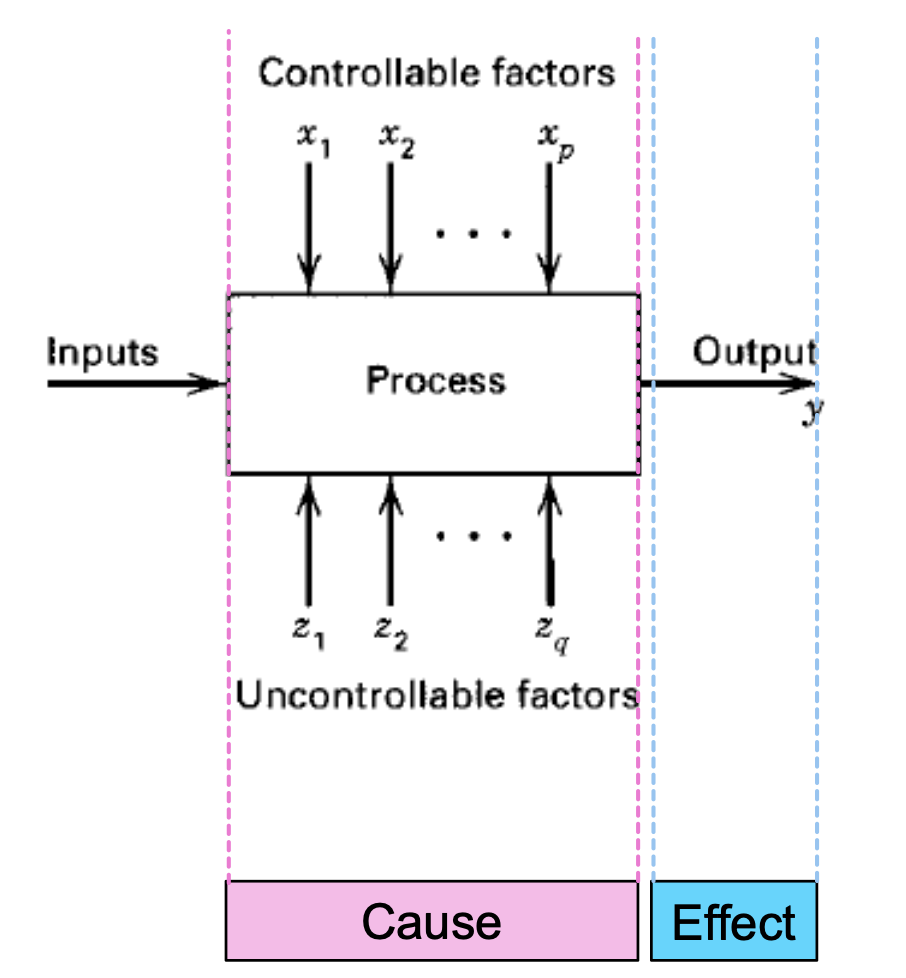
\includegraphics[width=0.4\linewidth]{cause-effect.png}
\end{center}


\subsection{Experimental Studies}

Before designing an experimental study, we must have a precise research question that is actually testable, i.e., that we can do the appropriate interventions and that we can measure the right response. \medskip

An experimental study consists of:

\begin{itemize}
	\item \textbf{Treatments / Predictors}: the different interventions on the system
	\item \textbf{Experimental units}: the actual objects on which we apply the treatments
	\item A method that assigns experimental units to treatments, typically \textbf{randomization}
	\item \textbf{Response(s)}: the output that we measure
\end{itemize}

\subsubsection{Treatments or Predictors}

We distinguish between the following types of predictors:

\begin{itemize}
	\item Predictors that are of primary interest and that can (ideally) be varied according to our “wishes”
	\item Predictors that are systematically recorded such that potential effects can later be eliminated in our calculations (\textbf{covariates})
	\item Predictors that can be kept constant and whose effects are therefore eliminated
	\item Predictors that we can neither record nor keep constant
\end{itemize}

\subsubsection{Randomization}

Randomization ensures that the only systematic difference between the groups is the treatment. This protects us from confounders and is the reason why a properly randomized experiment allows us to make a statement about a cause-effect relationship between treatment and response. Typically, we do a randomization “within” homogeneous blocks. This restricted version of randomization is called \textbf{blocking}. A block is a subset of experimental units that is more homogeneous than the entire set.

\subsubsection{Experimental and Measurement Units}

An \textbf{experimental unit} is defined as the object on which we apply the treatments by randomization. On the other hand, a \textbf{measurement unit} is the object on which the response is being measured. They do not have to be the same.

\subsubsection{Experimental Error}

Different experimental units will give different responses to the same treatment (\textbf{experimental error}). Therefore we need multiple replicates receiving the same treatment. If the difference between the treatments is much larger than the experimental error, we can conclude that there is a treatment effect.

\subsubsection{Blinding}

\textbf{Blinding} means that those who measure the response do not know which treatment is given. With humans it is common to use \textbf{double-blinding} where in addition the patients do not know the assignment either. Blinding protects us from (unintentional) bias due to expectations.

A \textbf{control treatment} is typically a standard treatment with which we want to compare. It can also be no treatment at all.
\section{Completely Randomized Design}

We assume for the moment that the experimental units are homogeneous. We know how to compare two independent groups using the two-sample t-test. If we have more than two groups, this is not applicable anymore.


\subsection{One-Way Analysis of Variance}

On an abstract level we want to compare $g \geq 2$ treatments, having $N$ experimental units, that we assign randomly to the different treatment groups having $n_i$ observations each. This is what we call \textbf{completely randomized design}, it is the most elementary experimental design. If all the treatment groups have the same number of experimental units, we call the design \textbf{balanced}.
\begin{lstlisting}
sample(treat.ord) ## Random Permutation of treat.ord
\end{lstlisting}

\subsubsection{Cell Means Model}

Let $y_{ij}$ be the observed response from the $j$-th experimental unit in treatment group $i$. In the \textbf{cells mean model} we allow each treatment group (cell) to have its own expected value. This means that $y_{ij}$ is the realised value of the random variable:
$$Y_{ij} \sim \mathcal N(\mu_i, \sigma^2), \; \text{ or } \; Y_{ij} = \mu_i + \epsilon_{ij}, \;\; \epsilon_{ij} \sim \mathcal N(0, \sigma^2)$$

As for the standard two-sample t-test, the variance is assumed to be equal for all groups. We say that $Y$ is the response and the treatment allocation is a categorical predictor. A categorical predictor is also called a factor. We sometimes distinguish between unordered (or nominal) and ordered (or ordinal) factors. We can rewrite the equation as:
$$\mu_i = \mu + \alpha_i$$

Where $\alpha_i$ is called the \textbf{treatment effect}. This will later help us to untangle the influence of multiple treatment factors on the response. Through this rewrite we have introduced an additional parameter, to remove it again we need a side constraint. Possible constraints could be:

\begin{itemize}
	\item weighted sum-to-zero: $\sum_{i=1}^{g} n_i \alpha_i = 0$
	\item sum-to-zero: $\sum_{i=0}^g a_i = 0$
	\item reference group: $\alpha_1 = 0$
\end{itemize}

For all of the choices it holds that $\mu$ determines some sort of "global level" of the data and $\alpha_i$ contains information about differences between the group means $\mu_i$ from that "global level". If we know $g-1$ of the $\alpha_i$, we automatically know the remaining $\alpha_i$, we also say that the treatment effect has $g-1$ \textbf{degrees of freedom} (df).

\begin{lstlisting}
## Options takes two args, the first for unordered 
## and the second for ordered factors.
## contr.poly        (weighted sum-to-zero) DEFAULT
## contr.sum         (sum-to-zero)
## contr.treatment (reference group)
options(contrasts = c("contr.sum", "contr.poly"))
\end{lstlisting}

\subsubsection{Parameter Estimation}

We estimate the parameters using the least squares criterion:
$$\hat \mu, \hat \alpha_i = \argmin{\mu, \alpha_i} \sum_{i=1}^g \sum_{j=1}^{n_i}(y_{ij} - \mu - \alpha_i)^2$$

Some notation:
\begin{align*}
	y_{i.} &= \sum_{j=1}^{n_i}y_{ij} 			  \qquad \qquad  \bar y_{i.} = \frac{1}{n_i}y_{i.}\\
	y_{..} &= \sum_{i=1}^g \sum_{j=1}^{n_i}y_{ij} \qquad \ \bar y_{i.} = \frac{1}{N} y_{..}
\end{align*}

As we can independently estimate the values of $\mu_i$, one can show that $\hat \mu_i = \bar y_{i.}$. From $\hat \alpha_i = \hat \mu_i - \hat \mu$ we can get all the other parameters needed (they still depend on the side constraint). \medskip

The estimate of the error variance is also called \textbf{mean squared error} $MS_E$:
$$\hat \sigma^2 = MS_E = \frac{1}{N - g} SS_E$$

Where $SS_E$ is the \textbf{error} or \textbf{residual sum of square}:
$$SS_E = \sum_{i=1}^g \sum_{j=1}^{n_i}(y_{ij} - \hat \mu_i)^2$$

Alternatively we can write this as:
$$MS_E = \frac{1}{N-g} \sum_{i=1}^g (n_i - 1) s_i^2, \qquad s_i^2 = \frac{1}{n_i -1} \sum_{j=1}^{n_i}(y_{ij} - \hat \mu_i)^2$$

Where $s_i^2$ is the empirical variance in treatment group $i$. The demoninator $N - g$ ensures that $\sigma^2$ is an unbiased estimator (the error estimate has $N-g$ degrees of freedom).

\begin{lstlisting}
fit <- aov(y ~ x, data = d)
## Get the estimated coefficients
coef(fit) ## or dummy.coef(fit)
## (Intercept) grouptrt1 grouptrt2
##       5.032      -0.371      0.494
\end{lstlisting}

\subsubsection{Tests}

With the two-sample t-test, we could test whether two samples share the same mean. We will now extend this for $g > 2$. Saying that all groups share the same mean is equivalent to saying:
$$Y_{ij} = \mu + \epsilon_{ij}, \; \; \epsilon_{ij} \sim \mathcal N(0, \sigma^2)$$

This is the so-called \textbf{single mean model}, a special case of the cell means model. We have the global null hypothesis
$$H_0 : \mu_1 = ... = \mu_g$$

therefore the alternative hypothesis is
$$H_A : \mu_k \neq \mu_l \text{ for at least one pair } k \neq l.$$

The idea is to check whether the variation between the different treatment groups (the "signal") is  larger than the variation within the groups (the "noise"). We can decompose the total variation as follows:
$$\underbrace{\sum_{i=1}^g \sum_{j=1}^{n_i}(\bar y_{ij} - \bar y_{..})^2}_{SS_T} = \underbrace{\sum_{i=1}^g \sum_{j=1}^{n_i}(\bar y_{i.} - \bar y_{..})^2}_{SS_{Trt}} + \underbrace{\sum_{i=1}^g \sum_{j=1}^{n_i}(y_{ij} - \hat \mu_i)^2}_{SS_E} $$

Where $SS_T$ is the total sum of squares, $SS_{Trt}$ the treatment sum of squares (between groups) and $SS_E$ the error sum of squares (within groups).\medskip

This information can be summarized in a \textbf{ANOVA} table.
\begin{center}
	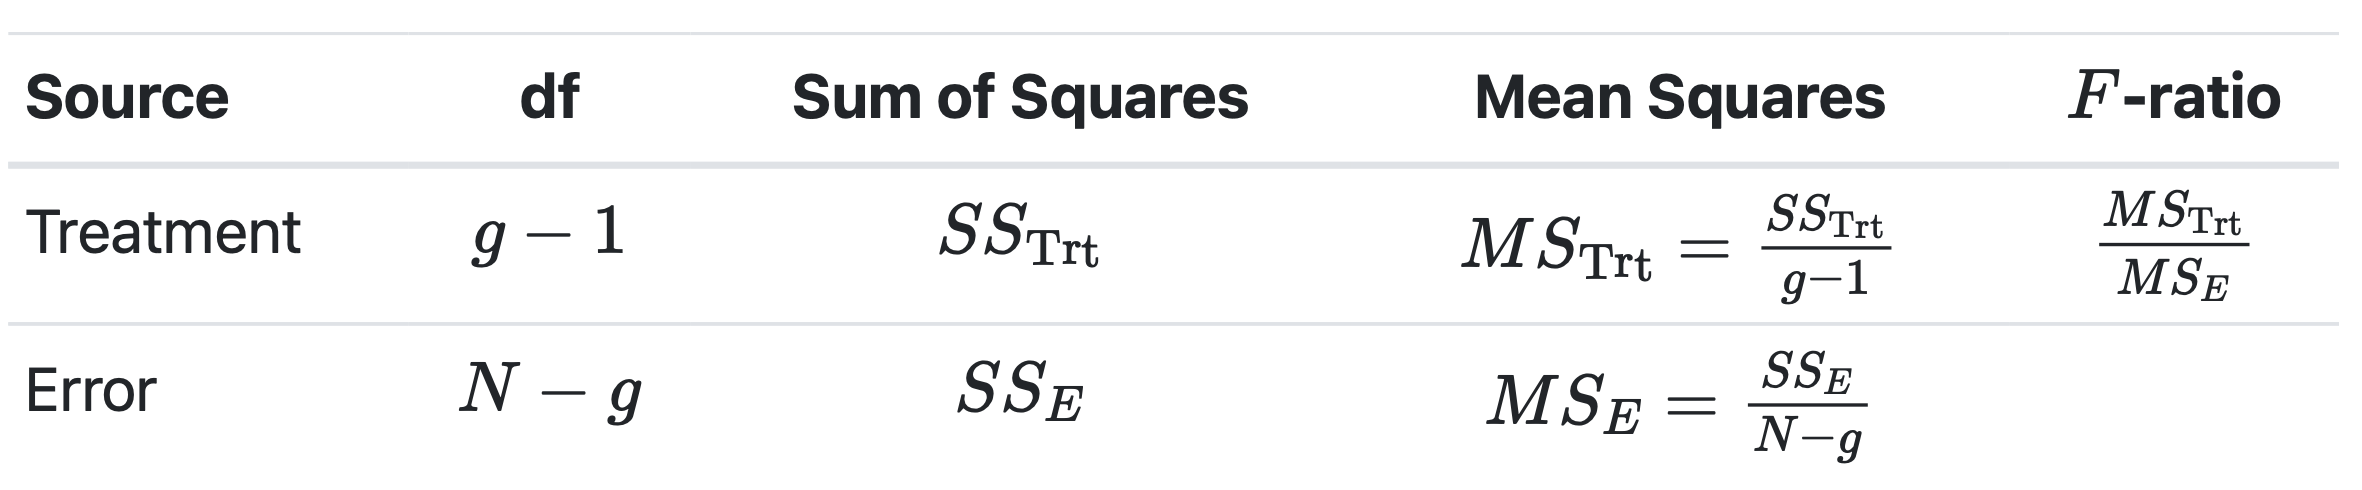
\includegraphics[width=\linewidth]{anova-table.png}
\end{center}

The $MS$ and $SS$ are normalized with the corresponding degrees of freedom. This is a so-called one-way ANOVA, because there is only one factor involved. If all groups share the same expected value, the treatment sum of squares is typically small. We introduce the so called $F$-ratio.
$$F\text{-ratio } = \frac{MS_{Trt}}{MS_E} \sim F_{g-1, N-g}$$

If the variation between groups is substantially larger than the variation within groups (higher $F$-ratio), we have evidence against $H_0$. The $F$-distribution looks as follows:
\begin{center}
	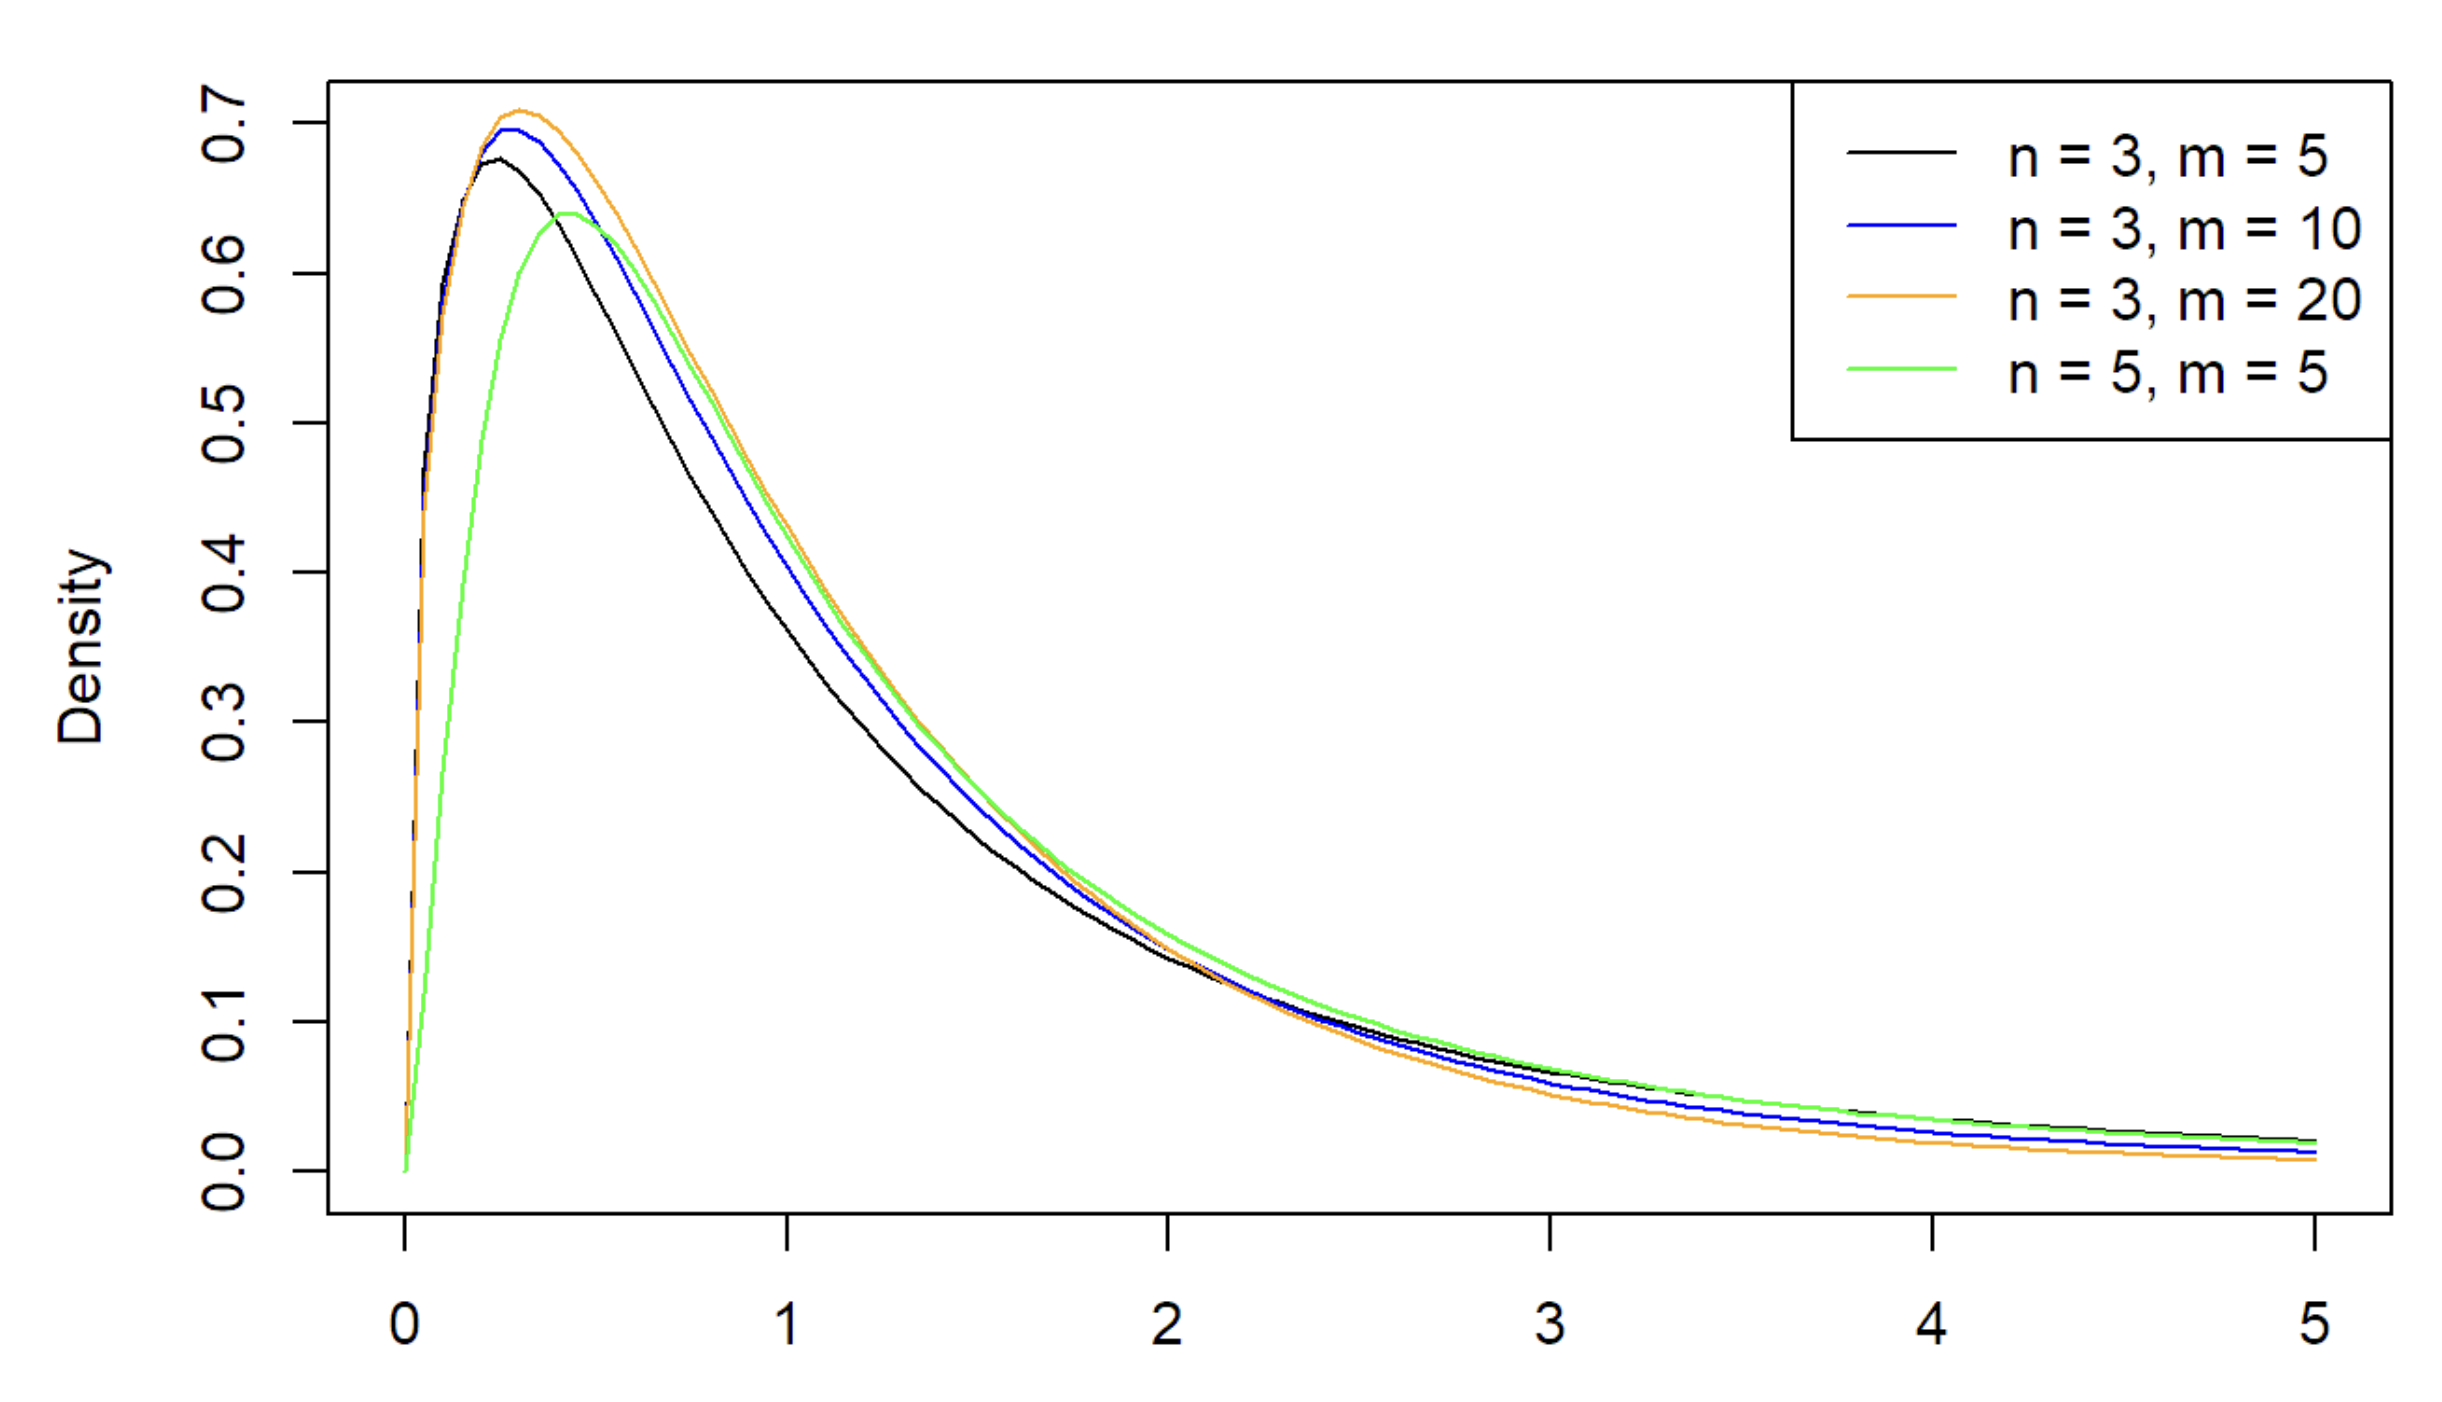
\includegraphics[width=0.8\linewidth]{f-distribution.png}
\end{center}

As with any other statistical test, we reject $H_0$ if the observed value of the $F$-ratio, our test statistics, lies in an "extreme" region of the corresponding $F$-distribution:
$$F \text{-ratio} > F_{g-1, N-g, 1 - \alpha}$$

Where $\alpha$ is often chosen as 0.05. Since this test is based on the $F$-ratio we call it an \textbf{$F$-test}.

\begin{lstlisting}
summary(fit)
##             Df Sum Sq Mean Sq F value Pr(>F)
## group        2   3.77    1.883     4.85   0.016
## Residuals   27  10.49    0.389
\end{lstlisting}

To perform statistical inference on the individual $\alpha_i$'s we use:
\begin{lstlisting}
summary.lm(fit)   ## for the tests
confint(fit)      ## for the confidence intervals
\end{lstlisting}


\subsection{Checking Model Assumptions}

Statistical inference is only valid if all model assumptions are fulfilled. So far this means:
\begin{itemize}
	\item The errors are independent
	\item The errors are normally distributed
	\item The error variance is constant
	\item The errors have mean zero
\end{itemize}

We now introduce different plots to check these assumptions. This means that we use graphical tools to perform qualitative checks.\medskip

The errors $\epsilon_{ij}$ cannot be observed, but the redisuduals $r_{ij} = y_{ij} - \hat \mu_{i}$ can be used as an estimate.

\subsubsection{QQ-Plot}

In a QQ-plot we plot the empirical quantiles of the residuals vs. the theoretical quantiles. The plot should show a more or less straight line if the normality assumption is correct.
\\[-20pt]
\begin{center}
	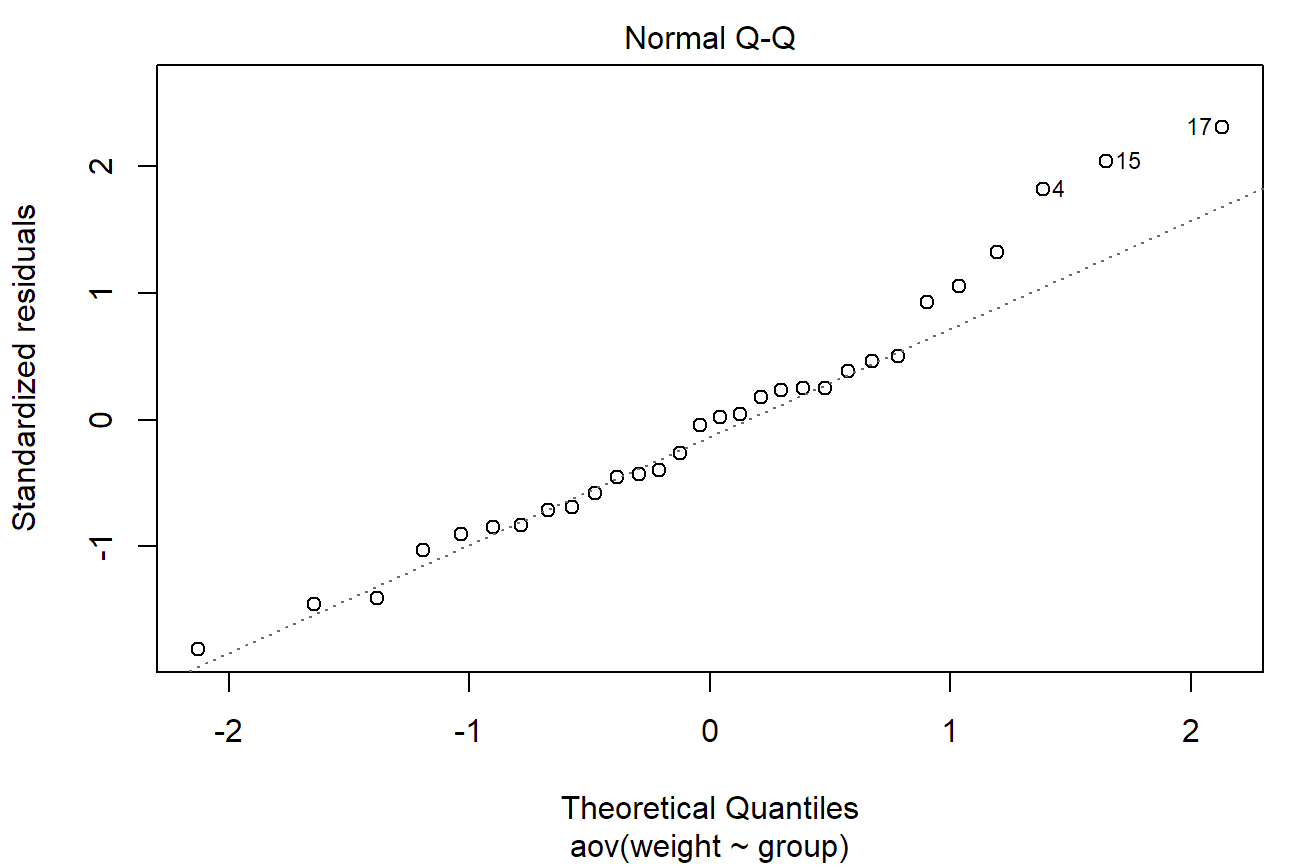
\includegraphics[width=0.8\linewidth]{qq-plot.png}
\end{center}
\begin{lstlisting}
plot(fit, which = 2)
\end{lstlisting}

\subsubsection{Tukey-Anscombe Plot}

The Tukey-Anscombe plot (TA-plot) plots the residuals $r_{ij}$ vs. the fitted values $\hat \mu_i$ (estimated cell means). It allows us to check whether the residuals have constant variance.
\begin{center}
	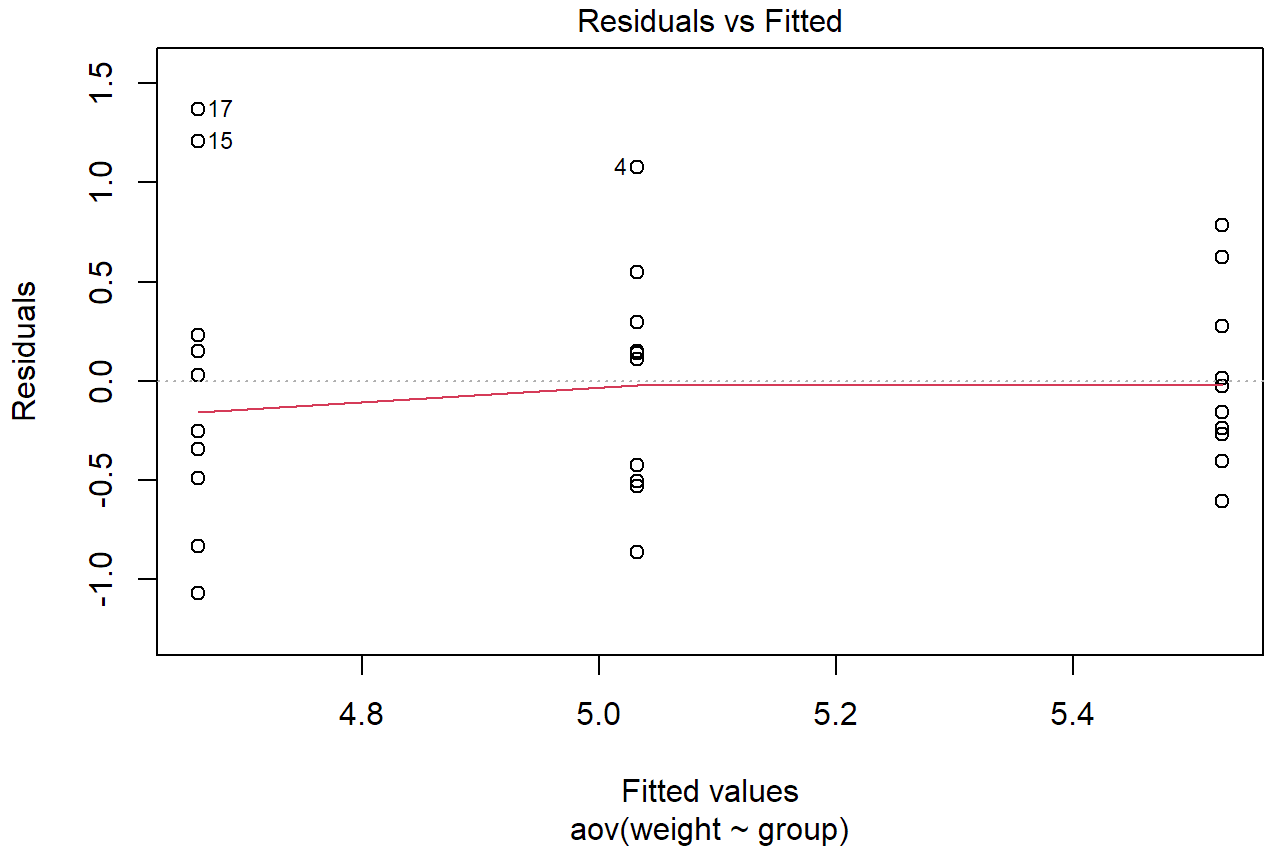
\includegraphics[width=0.8\linewidth]{ta-plot.png}
\end{center}
\begin{lstlisting}
plot(fit, which = 1)
\end{lstlisting}

\subsubsection{Index Plot}

If the data has some serial structure, i.e. a certain time order, we typically want to check whether residuals close in time are more similar than residuals far apart. For this we use the index plot. For positively dependent residuals, we would see time periods where most residuals have the same sign, while for negatively dependent residuals, the residuals would “jump” too often from positive to negative compared to independent residuals. 
\begin{center}
	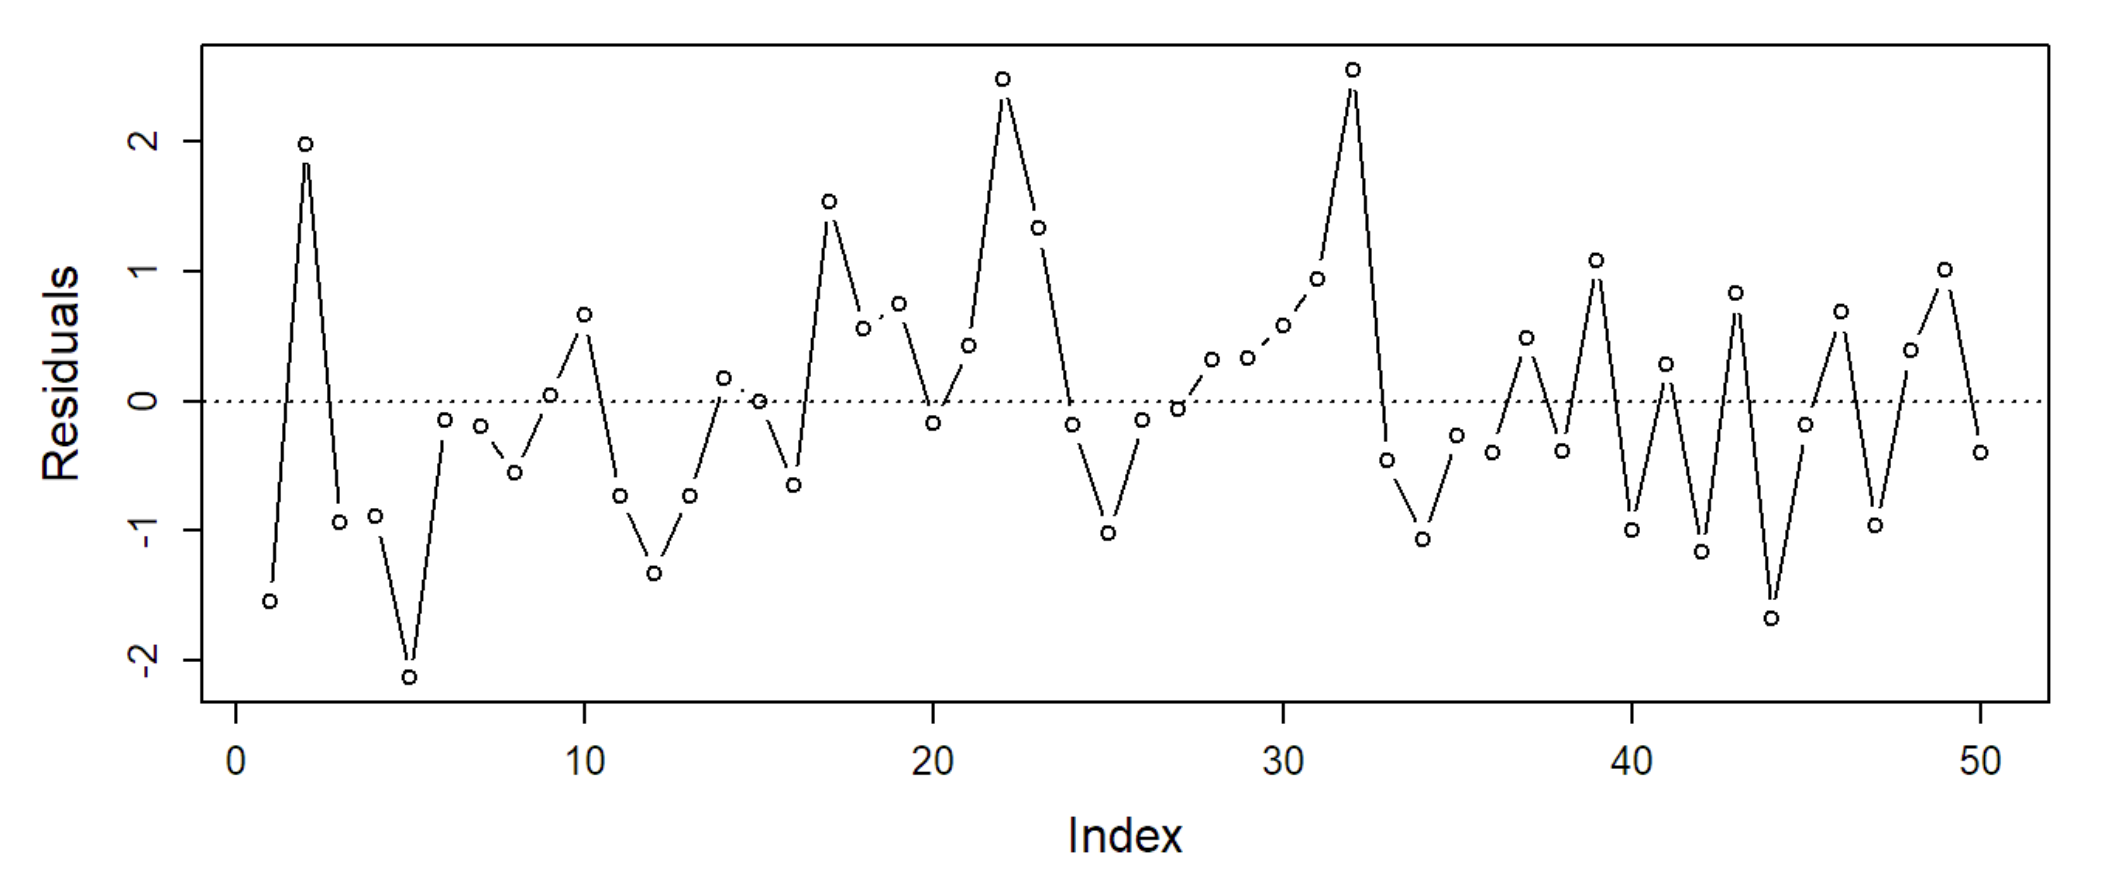
\includegraphics[width=\linewidth]{index-plot.png}
\end{center}


\subsubsection{Transformations Affect Interpretation}

Whenever we transform the response we implicitly also change the interpretation of the model parameters. Therefore, while it is conceptually attractive to model the problem on an appropriate scale of the response, this typically has the side effect of making interpretation more difficult. For example, if we use the logarithm:
$$\log (Y_{ij}) = \mu + \alpha_i + \epsilon_{ij}$$

All the $\alpha_i$ have to be interpreted on the log-scale. For example, if we us \textit{contr.treatment} and we have $\hat \alpha_2 = 1.5$. This means: on the log-scale we estimate that the average value of group 2 is 1.5 larger than the average value of group 1. What about the original scale? We know that $\E[\log(Y_{ij})] = \mu + \alpha_i$, but the expected value on the original scale does not directly follow the transformation. However, we can make a statement about the median. On the log-scale the median is equal to the mean, hence:
$$\text{media}(\log(Y_{ij})) = \mu + \alpha_i$$

In contrast to the mean, any quantile directly transforms with a strictly monotone increasing function. As the median is nothing else than the 50\% quantile, we have:
$$\text{media}(Y_{ij}) = e^{\mu + \alpha_i}$$

Similarly, for the ratio:
$$\frac{\text{media}(Y_{2j})}{\text{media}(Y_{1j})} = \frac{e^{\mu + \alpha_2}}{e^{\mu}} = e^{\alpha_2}$$

Hence, we can make a statement that on the original scale the median of group 2 is $e^{\alpha_2} = 4.48$ as large as the median of group 1. This means that additive effects on the log-scale become multiplicative effects on the original scale. Unfortunately, the statement is only about the median and not the mean on the original scale. \medskip

If we also consider a confidence intervals for $\alpha_2$, e.g. [1.2, 1.8], the transformed version [$e^{1.2}, e^{1.8}$] is a confidence interval for $e^{\alpha_2}$ which is the ratio of medians on the original scale.

\subsection{Power / What Sample Size Do I Need?}

By construction, a statistical test controls the so-called type I error rate with the significance level $\alpha$. This means that the probability that we falsely reject $H_0$ is less than or equal to $\alpha$. Besides the type I error, there is also a type II error. It occurs if we fail to reject $H_0$ even though $H_A$ holds. The probability of a type II error is typically denoted by $\beta$. \medskip

The \textbf{power} of a statistical test is defined as 
$$\text{P}(\text{reject } H_0 \; | \; \text{a certain setting under } H_A \text{ holds}) = 1 - \beta.$$

Intuitively, it seems clear that the "further away" we choose the parameter setting from $H_0$ the larger will be the power, or the smaller will be the probability of a type II error.

\subsubsection{Calculating Power for a Certain Design}

Power can be thought of as the probability of success, i.e. getting a significant result. The question of "what sample size do I need?" depends on the question of "what power do I want". The power depends on:
\begin{itemize}
	\item design of the experiment
	\item significance level
	\item parameter setting under the alternative
	\item sample size
\end{itemize}

We mainly use sample size and experimental design to maximize the power. Instead of doing the exact calculations, we rather choose an alternative way. We can always simulate a lot of data sets under $H_A$ that we believe in and check how often we are rejecting the corresponding $H_0$. The empirical rejection rate is then an estimate of the power. A nice side effect of doing a power analysis is that you actually do the whole data analysis on simulated data and you immediately see whether it works as intended. From a conceptual point of view, we can use such a simulation-based procedure for any design. However, the number of parameters grows rather quickly with increasing model complexity. \medskip

In that sense, the results of a power analysis are typically not very precise. However, they should still give us a rough idea about the required sample size in the sense of whether we need 6 or 60 observations per group.

\begin{lstlisting}
mu <- c(57, 63, rep(60, 3)) 
sigma2 <- 7 

## This will give us the estimated power
power.anova.test(groups = length(mu), n = 4, between.var = var(mu), within.var = sigma2)

## We can replace the argument n with power to get 
## and estimate for the needed sample size per group
power.anova.test(groups = length(mu), between.var = var(mu), within.var = sigma2, power = 0.8)
\end{lstlisting}

\section{Contrast and Multiple Testing}

\subsection{Contrast}

The $F$-test is rather unspecific and gives us basically a yes/no answer. It does not tell us what treatment (or combination of treatments) is significant. Such kind of questions can be formulated as so-called \textbf{contrasts}. As hypothesis we choose:
$$H_0 : \sum_{i=1}^g c_i \mu_i = 0 \text{ and } H_A : \sum_{i=1}^g c_i \mu_i \neq 0$$

Typically we have the side constraint that $\sum_{i=1}^g c_i = 0$. The contrast is about the differences between treatments and not about the overall response. We estimate the value of $\sum_{i=1}^g c_i \mu_i$ with:
$$\sum_{i=1}^g c_i \hat \mu_i = \sum_{i=1}^g c_i \bar y_{i.}$$

In addition, we could derive its accuracy (standard error), construct confidence intervals and do tests.

\begin{lstlisting}
library(multcomp)
## linfct is our contrast
fit.glht <- glht(fit, linfct = mcp(group = c(1, -1/2, -1/2)))
summary(fit.glht)
\end{lstlisting}

Every contrast has an associated sum of squares:
$$SS_C = \frac{(\sum_{i=1}^g c_i \bar y_{i.})^2}{\sum_{i=1}^g \frac{c_i^2}{n_i}}$$	

It has one degree of freedom and therefore $MS_C = SS_C$. We have:
$$\frac{MS_C}{MS_E} \sim F_{1, N-g}$$

Two contrasts $c, c^*$ are orthogonal if:
$$\sum_{i=1}^g \frac{c_i c_i^*}{n_i} = 0$$

In this case, the corresponding estimates are independent. If we have $g$ treatments, we can find
$g - 1$ different orthogonal contrasts (one dimension is already used by the global mean). A set of orthogonal contrasts partitions the treatment sum of squares meaning that if
$c^1, ..., c^{g-1}$ are orthogonal contrasts it holds that:
$$SS_{c^1} + ... + SS_{c^{g-1}} = SS_{Trt}$$

Multiple contrasts are all orthogonal if and only if for the matrix $C$ that represents them, $C^\top C$ is diagonal.


\subsection{Multiple Testing}

The problem with all statistical tests is the fact that the overall type I error rate increases with increasing number of tests. This means that if we perform many tests, we expect to find some significant results, even if all $H_0$ are true. Somehow we have to take into account the number of tests that we perform to control the overall type I error rate. \medskip

We list the potential outcomes of a total of $m$ tests, among which $m_0$ $H_0$ are true:
\begin{center}
	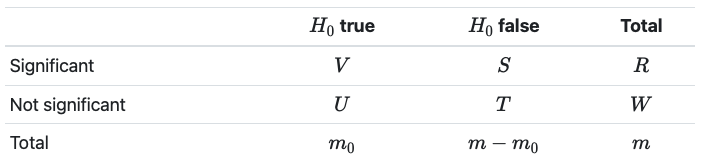
\includegraphics[width=\linewidth]{multiple_testing.png}
\end{center}

For example, $V$ is the number of wrongly rejected $H_0$ (type I errors, also known as FP). Using this notation, the overall or family-wise error rate (FWER) is defined as the probability of rejecting at least one of the true $H_0$'s:
$$\text{FWER} = P(V \geq 1)$$

The family-wise error rate is very strict in the sense that we are just interested in whether there is at least one wrong rejection. We say that a procedure controls the family-wise error rate in the strong sense at level $\alpha$ if FWER $\leq \alpha$ for any configuration of true and non-true $H_0$'s. \medskip

Another error rate is the FDR which is the expected fraction of false discoveries:
$$\text{FDR} = E \left[ \frac{V}{R} \right]$$

Controlling FDR at level $0.2$ means that on average in our list of significant findings only $20\%$ are false positives. If a procedure controls FWER at level $\alpha$, FDR is automatically controlled at level $\alpha$ too. This does not hold the other way around. \medskip

We can also control the error rates for confidence intervals. We call a set of confidence intervals simultaneous confidence intervals at level $(1 - \alpha)$ if the probability that all intervals cover the corresponding true parameter value is $(1 - \alpha)$. This means that we can look at all confidence intervals at the same time and get the correct “big picture” with probability $(1 - \alpha)$. \medskip

In the following, we typically start with individual p-values (the ordinary p-values corresponding to the $H_{0,j}$'s) and modify them such that the appropriate overall error rate (like FWER) is being controlled. The modified p-values should be interpreted as the smallest overall error rate such that we can reject the corresponding null hypothesis.

\subsubsection{Bonferroni}

The Bonferroni correction is a very generic but conservative approach. The idea is to use a more restrictive (individual) significance level of $\alpha^* = \alpha / m$. This procedure controls the FWER in the strong sense for any dependency structure of the different tests. Especially for large $m$, the Bonferroni correction is very conservative leading to low power.

\begin{lstlisting}
library(multcomp)
## K is a matrix with each row being a contrast
fit.glht = glht(fit, linfct = mcp(group = K))
summary(fit.glht, test = adjusted("bonferroni"))
\end{lstlisting}

\subsubsection{Bonferroni-Holm}

The Bonferroni-Holm procedure also controls the FWER in the strong sense. It is less conservative and uniformly more powerful, which means always better, than Bonferroni. It works in the following sequential way:
\begin{enumerate}
	\item Sort $p$-values from small to large
	\item For $j = 1,...$: Reject null hypothesis if $p_j \leq \frac{\alpha}{m-j+1}$
	\item Stop when reaching the first non-significant $p$-value and do not reject the remaining null hypotheses.
\end{enumerate}

Note that this procedure only works with p-values but cannot be used to construct confidence intervals.
\begin{lstlisting}
summary(fit.glht, test = adjusted("holm"))
\end{lstlisting}

\subsubsection{Scheffe}

The Scheffe procedure controls for the search over any possible contrast. This means we can try out as many contrasts as we like and still get honest p-values! This is even true for contrasts that are suggested by the data, which were not planned beforehand, but only after seeing some special structure in the data. The price for this is low power. \medskip

The Scheffe procedure works as follows: We start with the sum of squares of the contrast $SS_C$. Then we build the $F$-ratio:
$$\frac{SS_C/(g-1)}{MS_E}$$

\subsubsection{Tukey Honest Significant Differences}

A special case of a multiple testing problem is the comparison between all possible pairs of treatments. The output is a matrix of $p$-values of the corresponding comparisons. We could now use the Bonferroni correction method. However, there exists a better, more powerful alternative which is called Tukey Honest Significant Differences (HSD). \medskip

Think of a procedure that is custom tailored for the situation where we want to do a comparison between all possible pairs of treatments. We get both $p$-values (which are adjusted such that the family-wise error rate is being controlled) and simultaneous confidence intervals.
\begin{lstlisting}
TukeyHSD(fit)
\end{lstlisting}


\subsubsection{Multiple Comparisons with a Control}

 if we want to compare all treatment groups with a control group, we have a so-called multiple comparisons with a control (MCC) problem. The corresponding custom-tailored procedure is called Dunnett procedure. It controls the family-wise error rate in the strong sense and produces simultaneous confidence intervals. 
 
\begin{lstlisting}
fit.glht <- glht(fit, linfct = mcp(group = "Dunnett"))
summary(plant.glht)
\end{lstlisting}

 We get smaller $p$-values than with the Tukey HSD procedure because we have to correct for less tests; there are more comparisons between pairs than there are comparisons to the control treatment.


\end{multicols*}
\end{document}

% ____ FOOTER ______________________________________________________
% Content and Template: 
% original by Danny Camenisch (dcamenisch@inf.ethz.ch), 2022
% based on different summaries from many helpful people
